\documentclass[dvipsnames, svgnames, x11names,border=3pt]{standalone}
\usepackage{tikz,pgfplots}
\usepgfplotslibrary{fillbetween}
\usetikzlibrary{patterns}
\pgfplotsset{compat = 1.18,width=10cm, height=10cm}

\begin{document}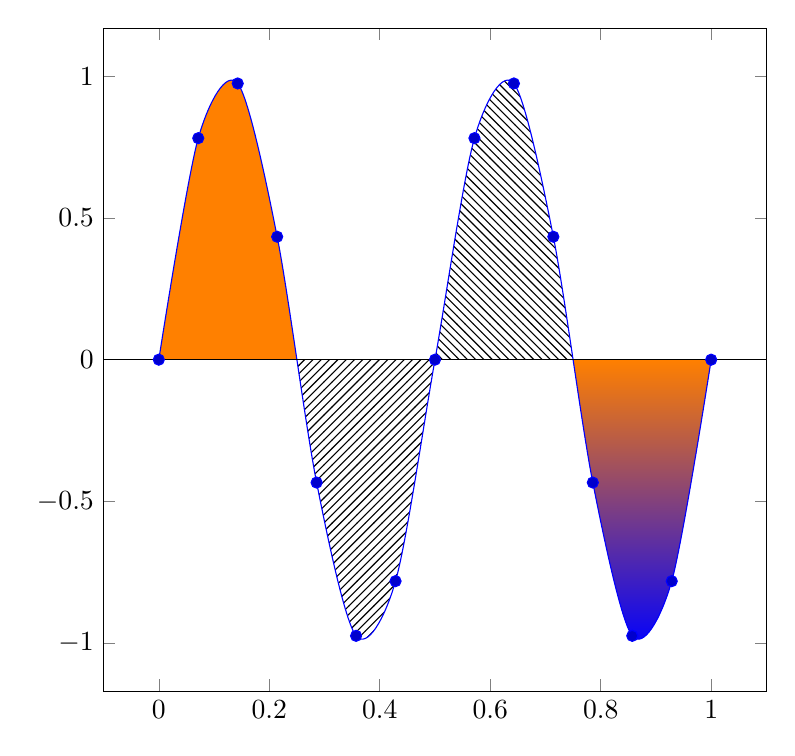
\begin{tikzpicture}\begin{axis}

\addplot+ [name path=A,samples=15,smooth,domain=0:1] {sin(720*x)};

\path [name path=B,draw]
(axis description cs:0,0.5)-- (axis description cs:1,0.5)
;

\addplot fill between [of=A and B,
    split,
    every segment no 0/.style={orange},
    every segment no 1/.style={pattern=north east lines},
    every segment no 2/.style={pattern=north west lines},
    every segment no 3/.style={top color=orange, bottom color=blue},
];

\end{axis}\end{tikzpicture}\end{document}
